%%%%%%%%%%%%%%%%%%
%%% QUESTION 4 %%%
%%%%%%%%%%%%%%%%%%
%TODO Question4
\clearpage		% page break
\question{}\label{q4}
%\partQuestion{}


		\begin{figure}[H] % H means, to put figure here after the code
		\centering
		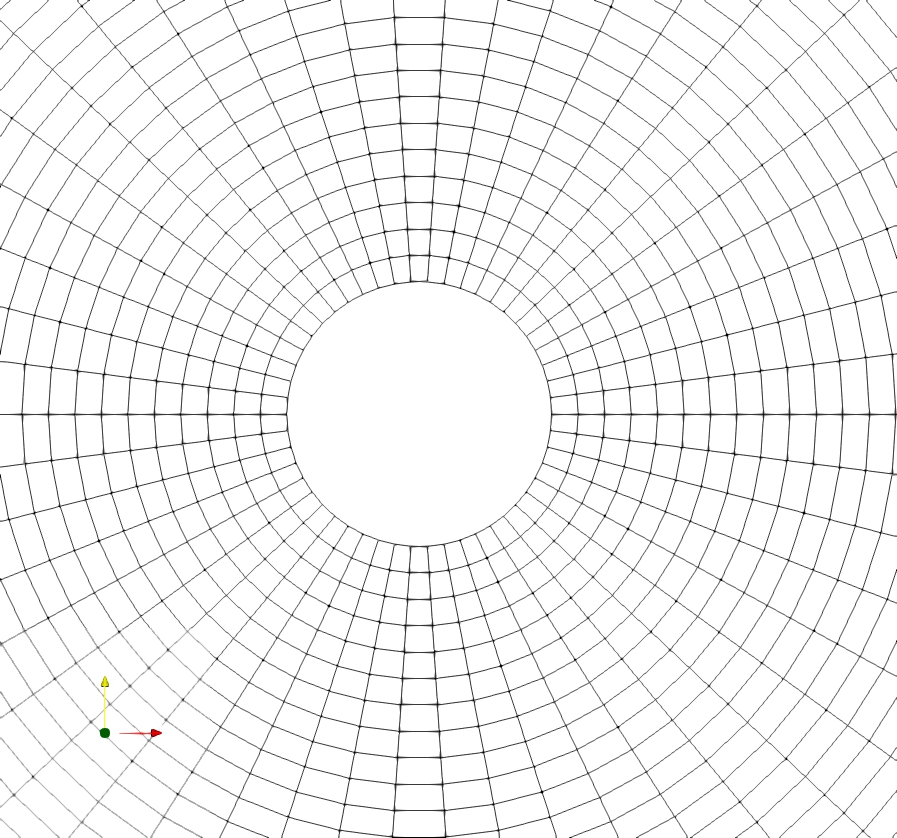
\includegraphics[width=0.75\textwidth, height=0.5\textwidth]{cylinderGrid-1}
		\caption{\rajah}
		\label{fig:cylinder}
	    \end{figure}	

The curvilinear boundary fitted grid as shown in \textbf{Figure \ref{fig:cylinder}}
is generated analytically using the equations below with $r_{0}$ as the radius of the cylinder. Answer the questions below regarding coordinate transformation.

\begin{subequations}
\begin{align}
x(r, \theta) &= (r_{0} + r) \cos \theta \nonumber  \\ \nonumber
y(r, \theta) &= (r_{0} + r)\sin \theta
\end{align}
\end{subequations}
		
\listbeginx	% start 1st level question

\item For each coordinate, the metrics are given as $x_{r}$, $y_{r}$, $x_{\theta}$ and $y_{\theta}$, where the subscript refers to partial derivatives. These metrics are required to transform any physical quantity derivative, for example $u_{x}$, into the computational domain derivatives of $u_{r}$ and $u_{\theta}$. Construct the projection of $u_{x}$ into domain $(r, \theta)$ using the metrics and $(u_{r},u_{\theta})$. 

\translation {Untuk setiap koordinat, metrik-metrik diberikan sebagai $x_{r}$, $y_{r}$, $x_{\theta}$ dan $y_{\theta}$, dimana subskrip merujuk kepada terbitan separa. Metrik-metrik ini diperlukan untuk mengubah apa-apa terbitan kuantiti fizik seperti $u_{x}$ untuk terma terbitan di domain pengiraan $u_{r}$ dan $u_{\theta}$. Binakan unjuran $u_{x}$ ke domain $(r, \theta)$ menggunakan metric-metric dan $(u_{r},u_{\theta})$. }
		
\qmarks{10}

\clearpage
%\nextpage

\item \label{q4b} \textbf{Table \ref{table:cell}} shows a sample coordinate of a cell from the grid in \textbf{Figure \ref{fig:cylinder}}. The Jacobian metric, $\textbf{J}$ of any cell in the grid is given as the equation below. Calculate the area of the cell and interpret its relation to the Jacobian metric.

\translation {Jadual\ref{table:cell} menunjukkan sampel koordinat satu sel daripada grid seperti di Rajah\ref{fig:cylinder}. Metrik Jacobian $\textbf{J}$ bagi mana-mana sel dalam grid diberikan seperti persamaan di bawah. Kirakan luas kawasan sel tersebut dan interpretasikan hubungannya dengan metric Jacobian.}

\begin{equation}
\textbf{J} = \det\begin{pmatrix} x_{r} & y_{r} \\ x_{\theta} & y_{\theta}  \end{pmatrix} = x_{r}y_{\theta} - x_{\theta}y_{r}
\end{equation}


\renewcommand{\arraystretch}{1.2}	% to make better spacing between rows
\begin{table}[H]
	\centering
	\caption{\jadual}	% no caption
	%	\begin{tabularx}{220pt}{c c}
	\begin{tabular}{|c|c|}
		%\toprule
		\hline
		%\toprule[1.5pt]
		\multicolumn{1}{|l|}{\textbf{x}} & \multicolumn{1}{l|}{\textbf{y}} \\
		\hline
0.927051 & 2.85317 \\
0.562144 & 2.94686 \\
0.988854 & 3.04338 \\
0.59962 & 3.14332 \\
		\hline
		%\bottomrule
		%\bottomrule[1.5pt]
	\end{tabular}
	%		\end{tabularx}%
	\label{table:cell}%
\end{table}%
		
		
\qmarks{10}


\item Sketch the cell in Q\ref{q4}\ref{q4b} roughly and calculate the outward pointing unit normal vector on each of the cell's side.

\translation {Lakarkan secara kasar sel daripada Q\ref{q4}\ref{q4b} dan kirakan nilai unit vektor normal di setiap sisi sel. }
		
\qmarks{5}


\listclose	% close 1st level question

\clearpage